\section{GPU Implementation}
\label{sec:implementation}

This paper presents GPU implementations of the existing object
detection program using a popular computer vision technique
\cite{Niknejad12}.
Our contribution is distinguished from prior GPU implementations work
\cite{Chen11, Prisacariu09} in that we analyze the performance
characteristics of the object detection program to figure out what part
of the program should be accelerated using the GPU and our
implementations build on this analysis optimizing performance.

Note that this paper focuses on vehicle detection but the presented GPU
implementations and our technical contribution can be applied for other
object detection methods using HOG features and deformable models.

\subsection{Basic Understanding}
\label{sec:understanding}

In GPU programming, the GPU code and the input data typically need to be
copied from the host to the device memory before we launch a function,
\textit{a.k.a.}, a compute kernel, on the GPU.
The output data also needs to be copied back from the device to the host
memory so that the CPU can read them.
Hence the GPU-accelerated computation comes at the expense of the
offloading overhead.
Another shortcoming of the GPU is its relatively low operating frequency
as compared to the CPU due to the presence of a significant number of
compute cores.
These trade-offs must be addressed to benefit from GPU programming; it
is a complex undertaking for programmers to ascertain appropriate
computational blocks that can accelerate on the GPU.
Nonetheless this massively parallel computing architecture is becoming a
trend in the state of the art.
Given that GPUs outperform traditional multithreaded and multicore CPUs
in peak performance by an order of magnitude \cite{Kato13_2}, it is
worth exploring a more efficient way of GPU programming.
This paper provides a guideline of how to use GPUs in an efficient way
for vision-based object detection.

\subsection{Program Analysis}
\label{sec:analysis}

As aforementioned, the usage of the GPU depends highly on the program
structure.
If the program does not contain data-parallel compute-intensive blocks,
the GPU is not effective at all.
Therefore it is important to analyze the program prior to coding and
implementation.
The following is a summary of the program sequence for HOG-based object
detection using the deformable models.
The detailed procedure and algorithm description are presented in
\cite{Felzenszwalb10, Niknejad12}.

\begin{enumerate}
\item Load an input image.
\item Load the pre-defined object models.
\item Calculate HOG features for all resized variants of the input
      image, often referred to as a \textit{HOG pyramid}.
\item Calculate similarity scores for every set of the root/part filters
      and the resized HOG images.
\item Detect an object region based on a summation of the similarity
      scores.
\item Recognize an object based on the detection result.
\item Output the recognition result.
\end{enumerate}

\begin{figure}[t]
 \begin{center}
  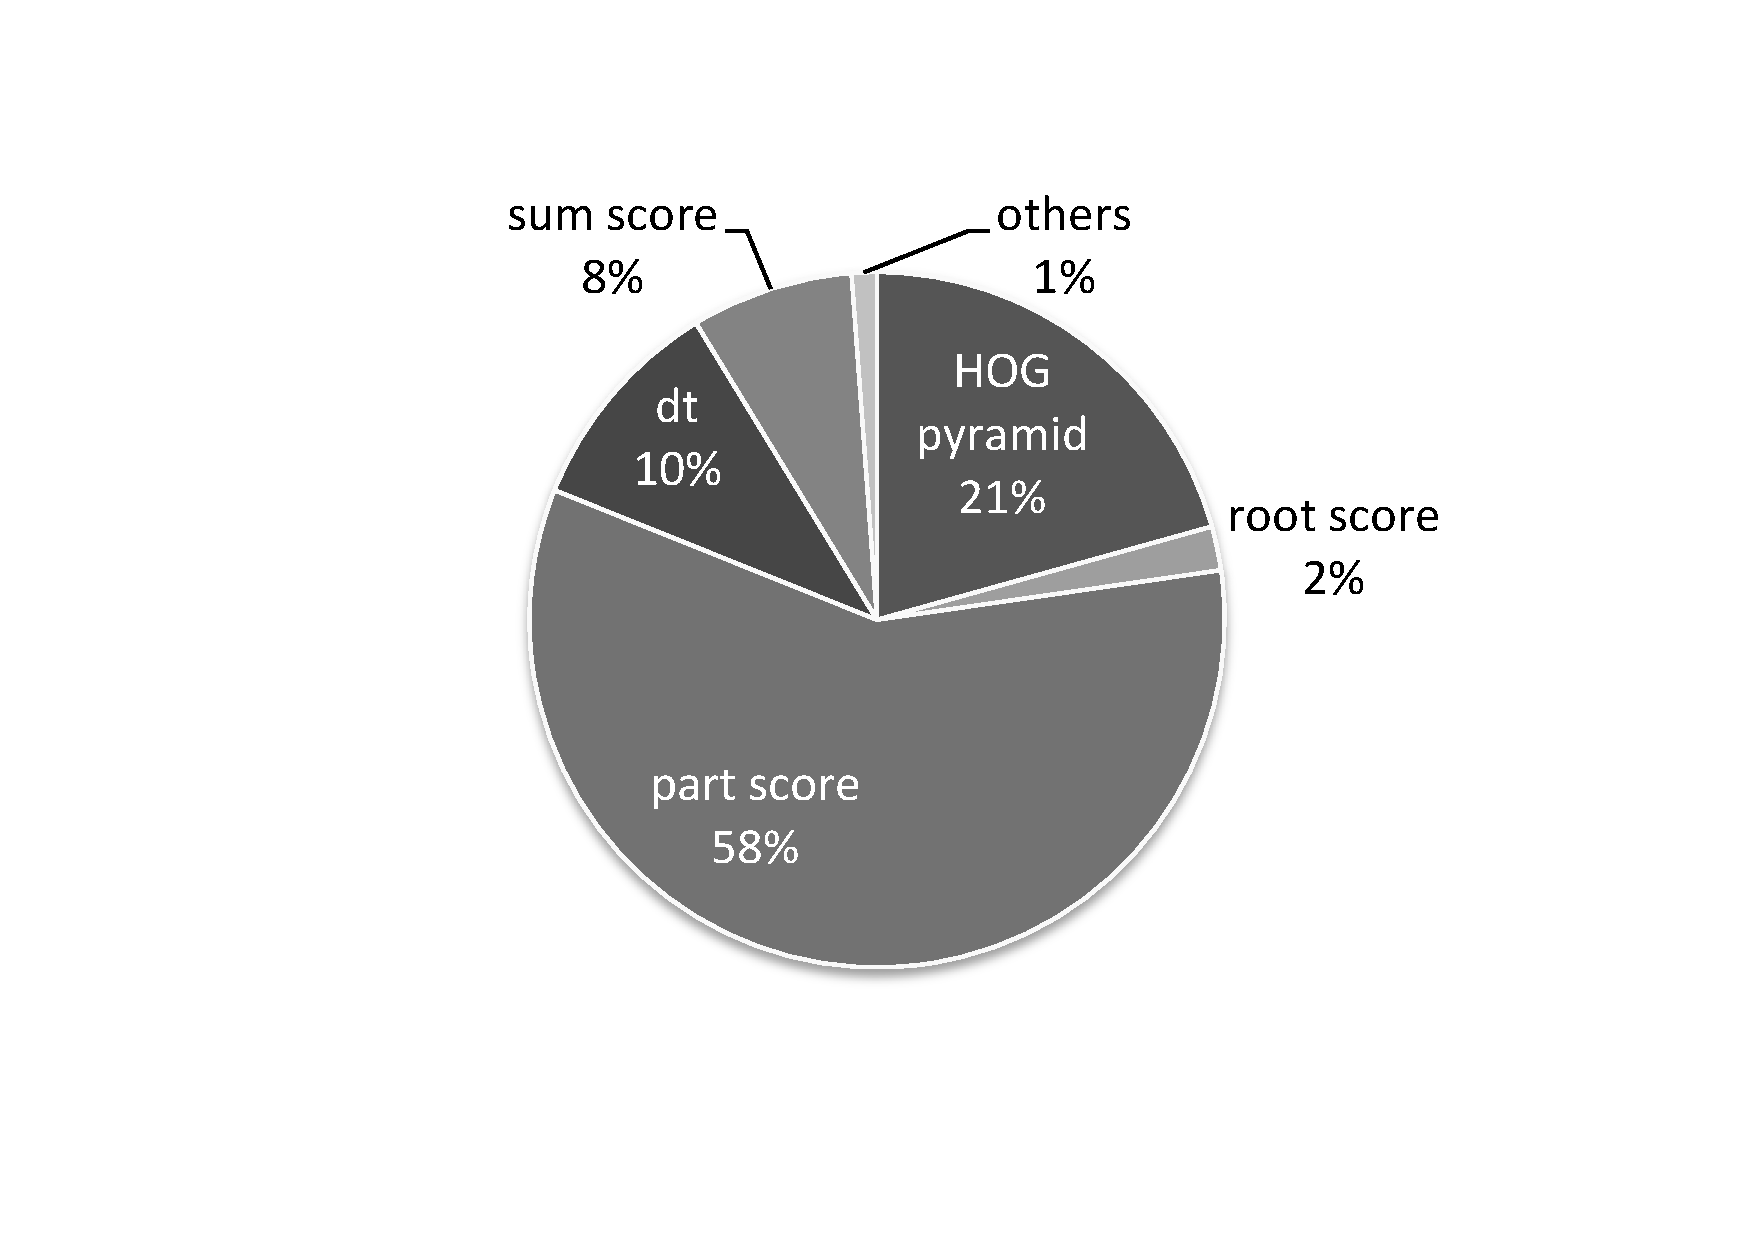
\includegraphics[width=\hsize]{fig/breakdown.pdf}\\
  \caption{The breakdown of computation times.}
  \label{fig:breakdown}
 \end{center}
\end{figure}

In order to identify computationally time-consuming blocks of the object
detection program, we conducted a preliminary measurement running the
original sequential code \cite{Niknejad12} on a generic Intel Core i7
2700K CPU.
The measurement method is straightforward.
We find high-level \textit{for} loops (in case that the program is
written in the C-like language) by scanning the program structure and
make a timestamp for each loop.
The result of measurement is shown in Fig.~\ref{fig:breakdown}.
Note that a label ``others'' represents the computation time excluding
the high-level \textit{for} loops.
This breakdown of computation times provides us with a hint of how to
approach GPU implementations.
Specifically an obvious computational bottleneck appears in the
calculation of similarity scores against the part filters, which
corresponds to partly ``Step 4)`` in the above program sequence.
This block dominates $58\%$ of the total time.
On the other hand, the calculation of HOG features corresponding ``Step
3)'' spends $21\%$ of the total time, while the detection and recognition
of the object, \textit{i.e.}, ``Step 5)'' and ``Step 6)'', contribute to
$10\%$ and $8\%$ of the total time respectively.

Our analysis conducted herein implies that even a simple time
measurement highlighting only the program structure without awareness of
the program context is helpful enough to understand computational
bottlenecks of the program.
In our case, it turned out that the most portion of the total time is
spent in the \textit{for} loops, which means that this program contains
a very high degree of parallelism and could be accelerated on the GPU.

\subsection{Implementation Approach}

We parallelize all the high-level \textit{for} loops of the program
using the GPU.
According to the measurement result in Fig.~\ref{fig:breakdown}, the
scoring of the root filters is a minor factor ($2\%$) of the total
time, but its program structure is almost identical to that of the part
filters and they adhere to continuous blocks.
Hence we include it to the GPU code.
In the rest of this section, we focus on the implementation of the
scoring of these filters, which is the most dominant part of the
program, due to a space constraint.

\begin{figure}[t]
 \begin{center}
  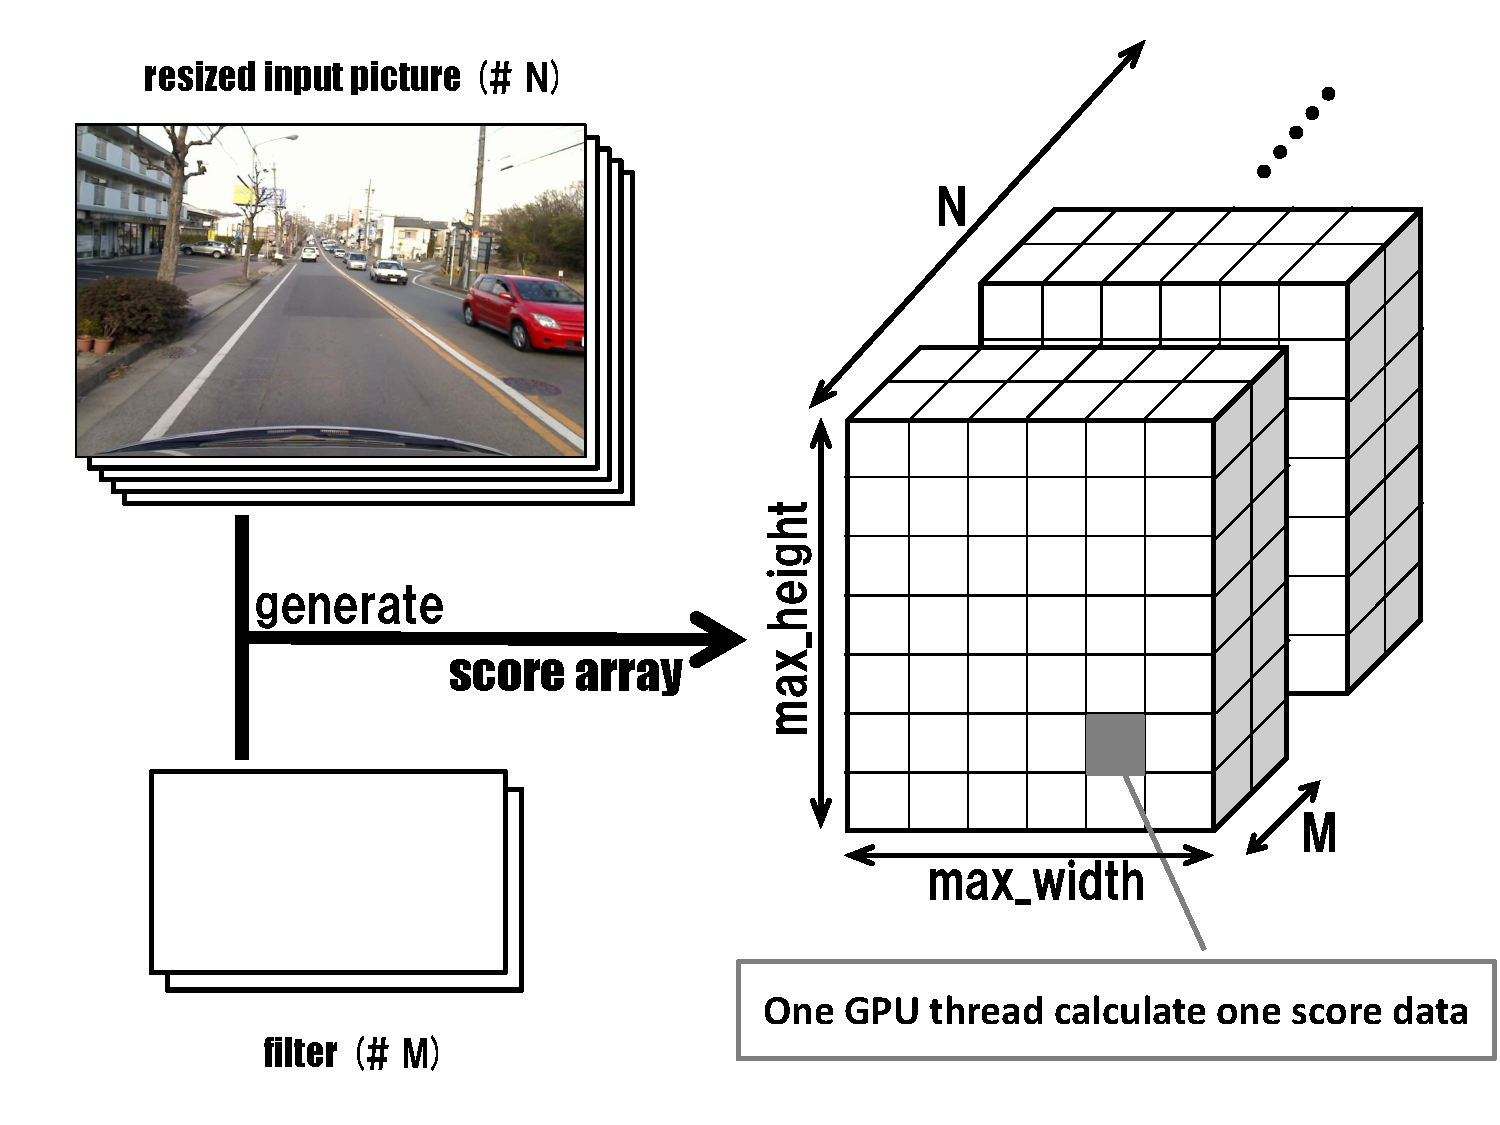
\includegraphics[width=\hsize]{fig/threads_shape.pdf}\\
  \caption{The number of compute threads and their block shape.}
  \label{fig:threads_shape}
 \end{center}
\end{figure}

Fig.~\ref{fig:threads_shape} illustrates a conceptual structure and flow
of our GPU implementation.
We have 32 resized pictures to be able to detect different sizes of the
object, \textit{i.e.}, \texttt{N} is 32.
We also have $2$ root filters and $12$ part filters to be able to detect
different shapes or angles of the object, \textit{i.e.}, \texttt{M} is 2
or 12.
A minimum piece of the similarity score for a HOG representation and an
object model can be calculated for each pixel of the filtered area
independently.
This area could be larger than a squire of $100$ pixels (equivalent to
\texttt{max\_width} $\times$ \texttt{max\_height}) for a $640 \times 480$
size of an image when using the trained data obtained from previous work
\cite{Niknejad12}.
Therefore the number of producible compute threads could be an order of
millions in this setup.
We shape these threads by blocks and grids for CUDA as shown in
Fig.~\ref{fig:threads_shape} where each block size is \texttt{max\_width}
$\times$ \texttt{max\_height} $\times$ \texttt{M} and each grid size is
\texttt{N}.
This shape is considered for ease of programming and a different shape
may further improve performance but such a fine-grained performance
tuning is outside the scope of this paper.

\subsection{GPU Programming}

Once computational blocks of the program to be parallelized are
determined, we can focus on the program structure rather than the
context when implementing the GPU code.
Listing~\ref{lst:score} illustrates a loop structure of the procedure
to score similarity of the input HOG image and the pre-defined object
models.
We find this structure containing fairly high parallelism, which means
that the impact of GPU implementations is significant, and apply the
implementation approach described in Fig.~\ref{fig:threads_shape}; the
depth of the third (\texttt{C\_height}) and the forth
(\texttt{C\_width}) loops is variable, and they could reach
\texttt{max\_height} and \texttt{max\_width} respectively.
Since these loops are independent with each other, we unroll all the
loops and assign all the elements of the iteration to millions of
individual threads on the GPU as shown in Fig.~\ref{fig:threads_shape}.

\begin{lstlisting}[caption=The program structure of similarity scoring, label=lst:score]
  for(int level=0; level<RESIZED_INPUT_NUM; level++) {
    for(int i=0; i<ROOTFILTER_NUM; i++) {
      for(int j=0; j<C_height; j++) {
        for(int k=0; k<C_width; k++) {
          .....
        }
      }
    }
    for(int i=0; i<PARTFILTER_NUM; i++) {
      for(int j=0; j<C_height; j++) {
        for(int k=0; k<C_width; k++) {
          .....
        }
      }
    }
  }
\end{lstlisting}

As aforementioned, GPU programming involes some trade-offs.
It is not straightforward to address these trade-offs due to a complex
architecture of the GPU.
For example, parallel threads may conflict on some functional unit.
Reducing the number of parallel threads mitigates this conflict but
results in less parallelism.
The best trade-off is obtained from optimized shapes of blocks and grids
depending on the GPU architecture.
We adopt comprehensive shapes of blocks and grids as presented in
Fig.~\ref{fig:threads_shape} because it simplifies programming while
still providing much better performance than CPU implementations.
An optimization of GPU programming is left open for future work.

Listing~\ref{lst:detect} illustrates the remainig parts of the program
that we parallelize using the GPU.
We also unroll all the loops of these blocks to accelerate computations
on the GPU.
Due to a space constraint, we skip the details of implementation approaches.

\begin{lstlisting}[caption=The program structure of region detection, label=lst:detect]
  for(int level=0; level<RESIZED_INPUT_NUM; level++) {
    for(int cmp; cmp<COMPONENT_NUM; cmp++) {
      for(int kk=0; kk<numpart[cmp]; kk++) {
        for(int x=0; x<dims[0]; x++) {
          ......
        }
        for(int y=0; y<dims[1]; y++) {
          ......
        }
        .....
      }
      sum_score(.....);
    }
  }
\end{lstlisting}